\documentclass{beamer}
\usetheme{Copenhagen}

\usepackage{booktabs}
\usepackage[brazil]{babel}

\title[Projeto de Rede Local]
{Projeto de Rede Local}

\subtitle{Campus Universitário}

\author[Auler, Tominaga, Sohngen, Aras] % (optional, for multiple authors)
{N.~V.~Auler\inst{1} \and B.~S.~Tominaga\inst{1} \and S.~Sohngen\inst{1} \and J.~P.~Aras\inst{1}}

\institute[Poli]
{
  \inst{1}%
  Engenharia de Computação\\
  Poli\--USP 
}

\date[Poli 2023]
{Redes de Computadores 2, Junho 2023}

\logo{
\includegraphics[height=1.2cm]{pcs.png}}

\begin{document}
\frame{\titlepage}

\begin{frame}
\frametitle{Table of Contents}
\tableofcontents[hideallsubsections]
\end{frame}

% add a section
\section[]{Laboratório de Sistemas Operacionais}

\begin{frame}
\frametitle{Laboratório de SO}
\framesubtitle{Pesquisa}
Inspirada no autor do livro de SO e criador do MINIX.

\begin{itemize}
    \item Protótipos de SO

        exemplos: MINIX 3, redox, serenity, fuchsia
    \item Inovação em SO

        exemplos: \textit{microkernel}, \textit{self-healing drivers} e \textit{userspace drivers}.
\end{itemize}

Aplicação será desenvolvida em um servidor de máquinas virtuais, com os seguintes objetivos:

\begin{itemize}
    \item Monitoramento das VM's, para que, até em caso das VM's falecerem, hypervisor colete dados
    \item Facilidade e padronização de ambiente
    \item Possibilidade de colaboração internacional (ex: Vrije)
\end{itemize}

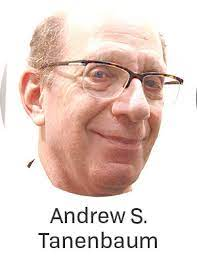
\includegraphics[width=0.15\textwidth]{tanem.jpg}
\end{frame}

\begin{frame}
\frametitle{Laboratório de SO}
\framesubtitle{QoS}

Quando trata\--se de VM's, deve\--se focar em Latência e Jitter, para nosso caso,
pois impacta a experiencia do usuário, além disso, no caso de cooperação internacional,
a latência não pode subir para algo inutilizável.

\begin{table}
  \centering
  \resizebox{10cm}{!}{
    \begin{tabular}{cccccc}
        \toprule
        Aplicações & Vazão & Latência & Jitter & Taxa de Erro & Disponibilidade\\
        & \footnotesize[Mbps] & \footnotesize[ms] & \footnotesize[ms] & \footnotesize[\%] & \footnotesize[\%]\\
        \midrule
        Hosting & $1000$ & $<10$ & $<5$ & $<1$ & ``3 nines''\\
        Monitoramento & $1-50$ & $<100$ & $<10$ & $<1$ & ``3 nines''\\
        \bottomrule
    \end{tabular}
    }
    \caption{Estimativas de QoS para a prototipagem de SO's.}
\end{table}
\end{frame}

\section[]{Laboratório de Computação Gráfica Distribuída}
\begin{frame}
\frametitle{Laboratório de Computação Gráfica Distribuída}
\framesubtitle{Aplicações de Pesquisa}
\begin{itemize}
\item{Engloba pesquisas em aplicações de renderização distribuída e simulação distribuída através da rede.}
\item{Foco em realizar pesquisas em aplicações gráficas utilizando concorrência, paralelismo e computação distribuída.}

\vspace{10pt}
\begin{columns}
% Column 1
\begin{column}{0.5\textwidth}
    \centering
    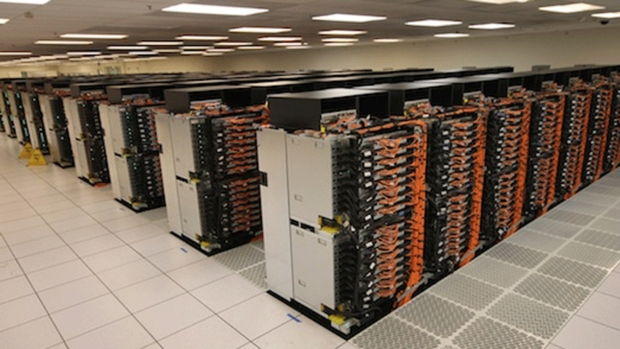
\includegraphics[width=0.9\textwidth]{compdist.png}
\end{column}
% Column 2    
\begin{column}{0.5\textwidth}
    \centering
    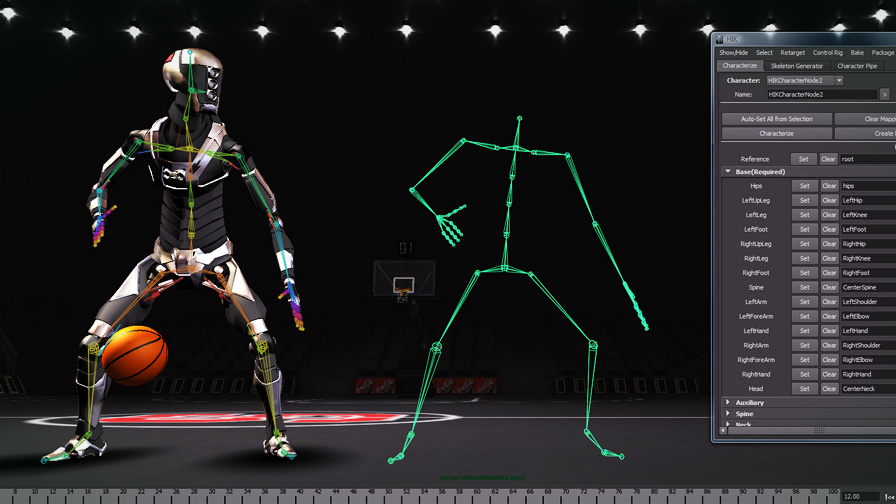
\includegraphics[width=0.9\textwidth]{rend.png}
\end{column}
\end{columns}

\end{itemize}
\end{frame}

\begin{frame}
\frametitle{Laboratório de Computação Gráfica Distribuída}
\framesubtitle{QoS}
\begin{table}
  \centering
  \resizebox{10cm}{!}{
    \begin{tabular}{cccccc}
        \toprule
        &\multicolumn{5}{c}{Parâmetros de Qualidade de Serviço} \\
        \cmidrule(rl){2-6}
        & Vazão & Latência & Jitter & Taxa de Erro & Disponibilidade\\
        Aplicações & [Mbps] & [ms] & [ms] & [\%] & [\%]\\
        \cmidrule(rl){1-6}
        Renderização distribuída & $10-100$ & $<50$ & Mínimo possível& $<1$ & $\approx100$\\
        \cmidrule(rl){1-6}
        Simulação distribuída & $1-100$ & $<100$ & $<10$ & $<1$ & $\approx100$\\
        \bottomrule
    \end{tabular}
    }
    \caption{Análise quantitativa de QoS para o Laboratório de Computação Gráfica Distribuída}
\end{table}
\end{frame}

\section[]{Laboratório de Machine Learning Distribuído}
\begin{frame}
\frametitle{Laboratório de Machine Learning Distribuído}
\framesubtitle{Aplicações de Pesquisa}
\begin{itemize}
\item{Aplicação centrada no aprendizado colaborativo, também conhecido como aprendizado federado, uma técnica de aprendizado de máquina que treina um algoritmo por meio de várias sessões independentes, cada uma usando seu próprio conjunto de dados conectadas por rede.}
\item{Pesquisa em otimização de modelos de maneira paralela e concorrente. Pode ser através de uma rede centralizada ou não.}
\end{itemize}
\end{frame}

\begin{frame}
\frametitle{Laboratório de Machine Learning Distribuído}
\framesubtitle{QoS}
\begin{table}
  \centering
  \resizebox{10cm}{!}{
    \begin{tabular}{cccccc}
        \toprule
        &\multicolumn{5}{c}{Parâmetros de Qualidade de Serviço} \\
        \cmidrule(rl){2-6}
        & Vazão & Latência & Jitter & Taxa de Erro & Disponibilidade\\
        Aplicações & [Mbps] & [ms] & [ms] & [\%] & [\%]\\
        \cmidrule(rl){1-6}
        Aprendizado federado & $10-100$ & $<100$ & $<15$ & $<1$ & $\approx100$\\
        \bottomrule
    \end{tabular}
    }
    \caption{Análise quantitativa de QoS para o Laboratório de Machine Learning Distribuído}
\end{table}
\end{frame}

\section[]{Laboratório de Eletrônica}
\begin{frame}
\frametitle{Laboratório de Eletrônica}
\framesubtitle{Aplicações de Pesquisa}
\begin{itemize}
\item{Pesquisa em dispositivos semicondutores e circuitos integrados}
\item{Energia Renovável}
\item{Segurança Eletrônica}
\end{itemize}
\end{frame}

\begin{frame}
\frametitle{Laboratório de Eletrônica}
\framesubtitle{QoS}
\begin{itemize}
\item{Pesquisa em dispositivos semicondutores e circuitos integrados}

    Vazão
\item{Energia Renovável}

    Latência, Vazão
\item{Segurança Eletrônica}

    Latência
\end{itemize}
\end{frame}

\end{document}
